%!TEX root = ../../thesis.tex

\section{Pipeline Comparison}
\label{sec:pipelines}
To transform the observed 2-D image from the telescope into an extracted 1-D spectrum of the target a number of steps (some outlined above in \cref{subsec:nirreduction}) have to be performed in sequence. The series of steps, performed by various software tools, is referred to as a \emph{pipeline}.
Each stage in the pipeline performs a specific task, for example creating the master dark frame, or performing the nod subtraction.
The result of one stage is passed to the next (either automatically or manually).
Two different pipelines were available to reduce the {CRIRES} observations used in this work.
The first is the standard {CRIRES} pipeline\footnote{\href{https://www.eso.org/sci/software/pipelines/}{https://www.eso.org/sci/software/pipelines/}}, available from {ESO}.
The second is an in-house pipeline previously used in~\citet{figueira_radial_2010} called {DRACS} (Data Reduction Algorithm for {CRIRES} Spectra)\change{Pedro it is my understanding that the {ESO} pipeline did not exist/was not publicly available when you created {DRACS}, correct?}. In these next sections the experience gained using both pipelines, comparing the extracted spectra and user experience is documented.


\subsection{{ESO} {CRIRES} pipeline}
\label{subsec:eso-crires}
The {ESO} {CRIRES} pipeline was used to reduce {CRIRES} nodding spectra following direction from the {CRIRES} pipeline user manual\footnote{\href{ftp://ftp.eso.org/pub/dfs/pipelines/crires/crire-pipeline-manual-1.13.pdf}{ftp://ftp.eso.org/pub/dfs/pipelines/crires/crire-pipeline-manual-1.13.pdf}} and the {CRIRES} reduction cookbook\footnote{\href{https://www.eso.org/sci/facilities/paranal/instruments/crires/doc/VLT-MAN-{ESO}-14200-4032\_v91.pdf}{https://www.eso.org/sci/facilities/paranal/instruments/crires/doc/VLT-MAN-{ESO}-14200-4032\_v91.pdf}}.

The GASGANO\footnote{\href{https://www.eso.org/sci/software/gasgano.html}{https://www.eso.org/sci/software/gasgano.html}} graphical user interface (GUI) was used to interact with the pipeline with guidance from the {GASGANO} manual\footnote{\href{https://www.eso.org/sci/software/gasgano/VLT-PRO-{ESO}-19000-1932-V4.pdf}{https://www.eso.org/sci/software/gasgano/VLT-PRO-{ESO}-19000-1932-V4.pdf}}.
This pipeline provides a number of \emph{recipes} which perform the required extraction steps.
From the GUI each recipe is manually selected, then the correct calibration and observation files need to be selected to use with each recipe.
The final output from the {ESO} pipeline is a table in a fits format with the combined extracted spectra (both \emph{rectangular} and \emph{optimal} extractions), pixel errors and a wavelength solution.

For a novice of spectral extraction this pipeline and the available documentation was very helpful to get started and perform the extraction.
However, to reduce many spectra it soon became a long tedious process.

Constant revision of the documentation was necessary to ensure all the correct image and calibration files were added to each recipe.
The {ESO} pipeline makes all the recipe parameters easily accessible to modify via a window of the recipe interface, but the recipe parameter defaults get restored for each observation, making it difficult to reduce all of the observations in a consistent manner.
Having the parameters adjustment on the recipe interface is great for adjusting the parameters and for identifying which parameters are relevant to each recipe.
Unfortunately, when trying to experiment with the recipe parameters to achieve a high quality spectral extraction it was repetitive to change the same parameters for each observation, and it was also difficult to keep track of all the changes while assessing their effect on the final output.

The parameters for the wavelength calibration were the most tedious.
To try and improve the wavelength calibration, the {y-positions} of the 6 \thar{} fibres were manually found from the images for each detector and every observation and then entered as input parameters for the calibration recipe.
This helped the wavelength calibration recipe to correctly identify/fit more of the \thar{} spectra in most cases, but this took time.
Because of this, it was chosen to use the other pipeline and these calibration were not used.

{ESO} has a new reduction ``workflow'' called {ESO} Reflex~\citep{freudling_automated_2013}\footnote{\href{https://www.eso.org/sci/software/esoreflex/}{https://www.eso.org/sci/software/esoreflex/}}.
This enables automated reduction with the ability to chain together the extraction recipes in the specific order desired, repeat steps to optimize the reduction, and automatically handle the data organization (no need to manually select the files for each recipe).
This would likely have enabled a quicker and more consistent reduction of the spectra.
Unfortunately, it is not available for the {CRIRES} pipeline.

\subsection{{DRACS}}
\label{subsec:dracs}
{DRACS} (Data Reduction Algorithm for {CRIRES} Spectra) is a custom reduction pipeline~\citep{figueira_radial_2010} written in {IRAF}'s CL\footnote{{IRAF} is distributed by the National Optical Astronomy Observatories, which are operated by the Association of Universities for Research in Astronomy, {Inc.}, under cooperative agreement with the National Science Foundation.}~\citep{tody_iraf_1993}.
It provides for automated dark and nonlinearity corrections (using the nonlinearity coefficients provided by {ESO}), as well as the flagging and replacement of bad pixels.
Sensitivity variations are corrected by dividing by a flat-field which was corrected from the blaze function effect.
The nodding pairs are mutually subtracted and the order tracing is accomplished by fitting cubic splines.
Order tracing allows the extraction algorithm to follow the shape for the dispersion across the detector\footnote{The spectra do not fall perfectly horizontally on the detector and usually contain some curvature due to the optics of the instruments.}.
By default the pipeline returns the \emph{optimal} extraction~\citep{horne_optimal_1986}, but the \emph{rectangular} extraction can also be obtained.
The extracted spectra from each nod is continuum normalized by dividing by a polynomial fitted to the continuum, with the polynomial degree selected individually for each spectrum and detector.
Finally, the normalized nod-cycle spectra are averaged together to give a single reduced spectrum, normalized to 1.

The {DRACS} pipeline was originally developed to work with \emph{H}-band spectra.
Because of this, some of the parameters were adjusted in an attempt to achieve a better reduction on the \emph{K}-band spectra analysed here.
The parameters adjusted were the tracing and normalization polynomial functions and their specific order on the detector.
Also, there was initially no reduction parameters present for detector \#3 as detector \#3 was not reduced in previous works using this pipeline.
Therefore, the pipeline was extended to be able to reduce detector \#3 of CRIRES, by adjusting the pipeline code and finding suitable parameters for detector \#3.

When using the {DRACS} pipeline on a new target, the tedious part is initially creating the lists of files identifying which files are the dark, flat, and the science frames\footnote{The {GASGANO} {GUI} was helpful to identify the distinction of each fits file for a beginner.}.
After these lists are created, the reduction pipeline can be run and re-run easily, making the effort worth it.

The first time through is interactive with a number of manual checks and decisions to be made (e.g.\ confirming the order tracing position, and fit is good).
{DRACS} remembers choices in a database, allowing for a reduced level of user interaction a second or third time through the pipeline.
This was useful to experiment with and iterate the reduction parameters of the pipeline.
When changing the parameters which affect the order tracing, the database with the order tracing results needed to be deleted so that it would not influence the new fits.
These parameters were therefore slower to iterate on.

This semi-autonomous nature of the {DRACS} pipeline means that all the spectra can be reduced in a consistent way, relatively quickly, and does not require manual spectra selection for each individual recipe as was done with the {ESO} pipeline.

There are a couple of drawbacks with using the {DRACS} pipeline.
The first is the lack of documentation on how to use it.
This required looking through the source code to find which functions and scripts do which part of the extraction.
{DRACS} makes use of many {IRAF} packages which have documentation available online\footnote{Such as at the \href{Space Telescope Science Institute}{http://stsdas.stsci.edu/gethelp/pkgindex\_noao.html}.}.
Searching through this documentation was difficult, but required, to understand how to use and modify {DRACS}.

The second drawback is that {DRACS} does not perform wavelength calibration, which is included with the {ESO} pipeline.
This means an external wavelength calibration was the only option (see \cref{subsec:wavecalib}).
The last drawback is the discovery of artefacts present in the nod spectra, which are discussed in detail in \cref{subsubsec:reductionartefacts}.

\subsection{Pipeline comparison and selection}
\label{subsec:pipeline-selection}
\begin{figure}
    \begin{tabular}{cc}
        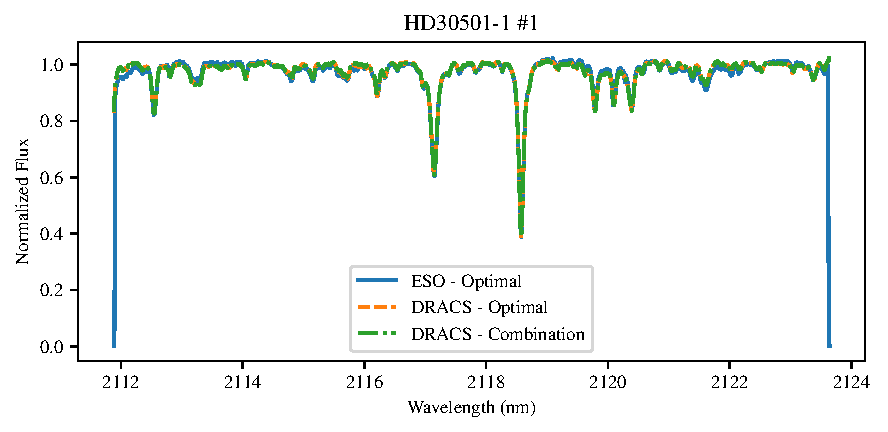
\includegraphics[width=0.5\linewidth]{figures/reduction/pipeline_compare/pipeline_compare_HD30501-1_chip_1} & 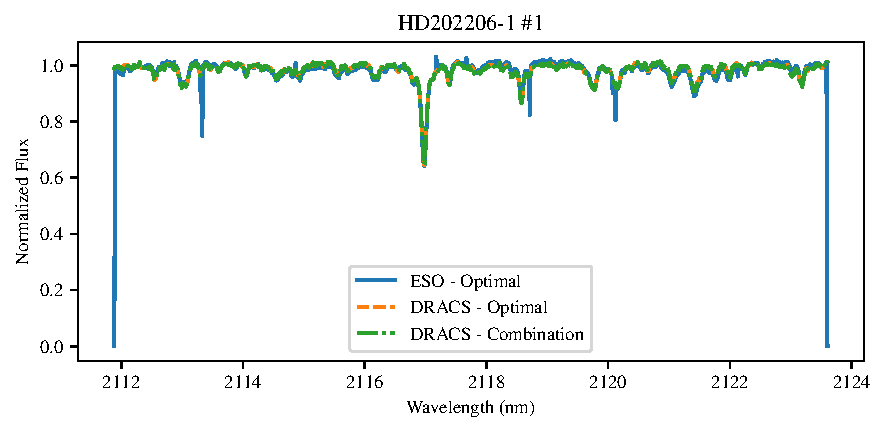
\includegraphics[width=0.5\linewidth]{figures/reduction/pipeline_compare/pipeline_compare_HD202206-1_chip_1}\\
        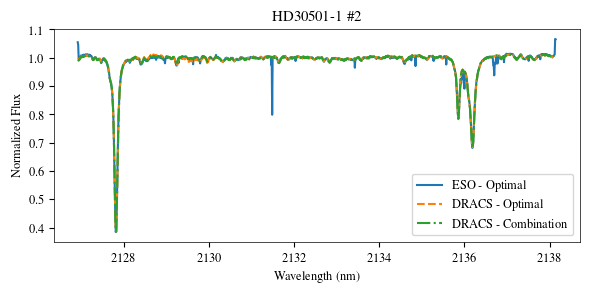
\includegraphics[width=0.5\linewidth]{figures/reduction/pipeline_compare/pipeline_compare_HD30501-1_chip_2} & 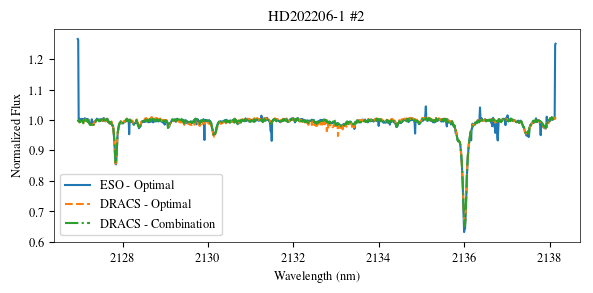
\includegraphics[width=0.5\linewidth]{figures/reduction/pipeline_compare/pipeline_compare_HD202206-1_chip_2}\\
        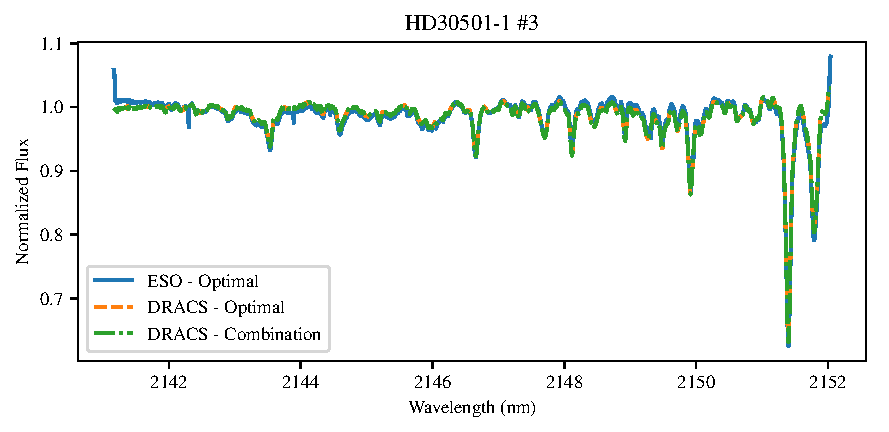
\includegraphics[width=0.5\linewidth]{figures/reduction/pipeline_compare/pipeline_compare_HD30501-1_chip_3} & 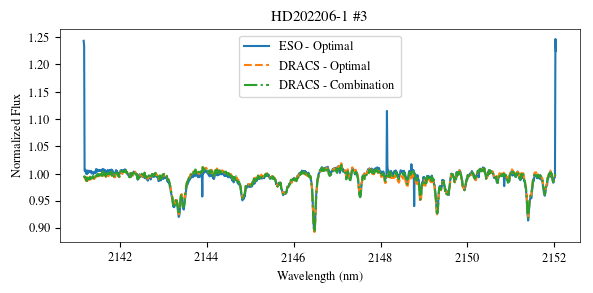
\includegraphics[width=0.5\linewidth]{figures/reduction/pipeline_compare/pipeline_compare_HD202206-1_chip_3}\\
        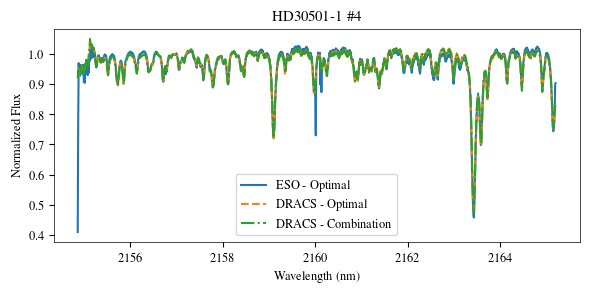
\includegraphics[width=0.5\linewidth]{figures/reduction/pipeline_compare/pipeline_compare_HD30501-1_chip_4} & 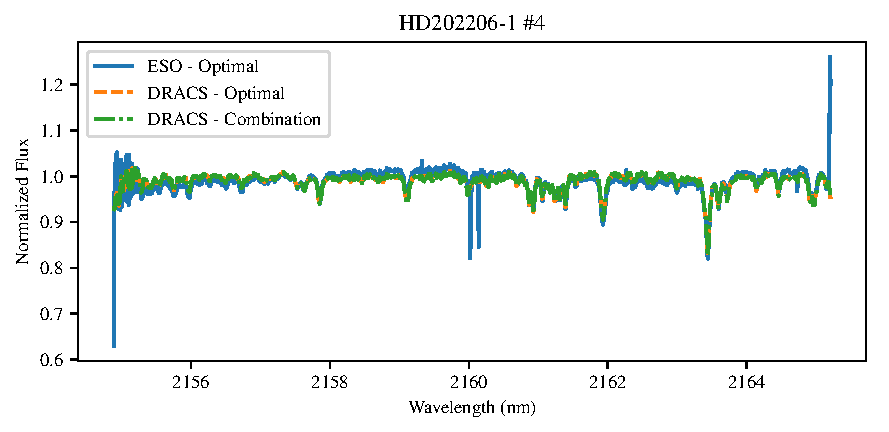
\includegraphics[width=0.5\linewidth]{figures/reduction/pipeline_compare/pipeline_compare_HD202206-1_chip_4}\\
    \end{tabular}
    \caption[Comparision between {DRACS} and {ESOs} reduction pipeline output.]{Comparison between the {ESO} pipeline and {DRACS} pipeline for two observations, {HD30501-1} and {HD202206-1}.
        The blue lines are the extracted spectra from the {ESO} pipeline, the orange dashed lines are the combined optimal extraction from the {DRACS} pipeline, and the green dash-dotted line is the modified {DRACS} extraction (after removing artefacts addressed in \cref{subsubsec:reductionartefacts}).
        The wavelength information applied to both spectra is from the {ESO} pipeline.}
    \label{fig:reduction-comparison}
\end{figure}

Both reduction methods were applied to the same {CRIRES} spectra to check the quality and consistency of both methods.
Two examples of the extraction for HD\,30501-1 (left) and HD\,202206-1 (right) from both pipelines are provided in \cref{fig:reduction-comparison}.
The blue lines are the extracted spectra from the {ESO} pipeline, the orange dashed lines are the optimal extraction from the {DRACS} pipeline, while the green dash-dotted line is the {DRACS} extraction after dealing with artefacts in the optimal extraction addressed in \cref{subsubsec:reductionartefacts}.

One of the important things checked was the line depths of each spectra to ensure that the pipelines were consistent.
The {ESO} pipeline has noticeable issues, with many large spikes still present in the spectra, likely caused by bad pixels or cosmic rays that are not correctly removed.
There also appears to be problems with the edges of the {ESO} reduced spectra, with very large spikes at either end.

At this stage the {DRACS} pipeline was chosen, as it was considered that the {DRACS} pipeline produced better extracted spectra than the {ESO} pipeline.
This decision was based on the quality of the reduced spectra, as well as the relative ease of use of the pipeline (being semi-automated once set up).
Another deciding factor was the need to create software to remove the bad pixels observed in the {ESO} reduced spectra.
However, this was unavoidable as it was eventually required for the {DRACS} reduced spectra (see \cref{subsubsec:reductionartefacts}).
Though the {ESO} pipeline provided a wavelength solution for the spectra, this did not factor into the decision as it was considered too unreliable due to known issues with {CRIRES} wavelength calibration, necessitating a new wavelength calibration anyway.

The spectra for the pipeline comparison in \cref{fig:reduction-comparison} are the combination of the 8 nod spectra.
Later, it was discovered that individual nod spectra from the {DRACS} pipeline had issues (see \cref{subsubsec:reductionartefacts}).
These are difficult to notice on this scale as they each constitute one eighth of the information in the combined spectrum.
An example of this is seen in detector \#2 of {HD202206-1} in \cref{fig:reduction-comparison}.
In \cref{fig:resizednods} an artefact from a single nod spectra, is barely visible in the pipeline comparison of \cref{fig:reduction-comparison}, shown as a slight depression of the orange dashed line between 2\,132 and 2\,134\nm{}.
The identification of these artefacts and how they are removed (green lines) are explained in the following section.

